\chapter{Methods} % Main chapter title
In this chapter we will discuss the methods used to achieve the objective of the research and why they are the best suited for the preveiously explained data  

\label{Chapter4}


\section {Human Intent Recognition}
As mentioned in the previous chapter, the most prominent features of human intent recognition were the two main categories of data, the first being the distance from the object and the second one beeing the direction of the end effector.
Another importsnt feature is the time, as the data is collected over time, it is important to take into account the time series nature of the data.
Given the nature of the data a valid approach could've been the one used in the paper , using HMM.\\
Although valid, having as trainable parameter only the rate parameter $\lambda$ of the exponential distribution, the introduction of hand tunable coefficients as the weight parameters for the observation probability, the model will result biased and will simplify the complex nuances of the human intention.
Since the need to comprehend the intrsinc connection between distance and direction and how this relation varies in time, a more sophidticated model was needed.\\
A novel approach in intent recognition is to use Recurrent Neural Networks, more specifically Long Short Term Memory Networks, a type of RNN that is capable of learning long-term dependencies.

\subsection{Recurrent Neural Networks}

A recurrent neural network (RNN) is a specialized form of artificial neural network designed to handle time series data or sequential data. 
Unlike standard feedforward neural networks, which assume that data points are independent of each other, RNNs are tailored for scenarios where the relationship between sequential data points is crucial. 
In such cases, where one data point is dependent on the previous ones, the neural network architecture must be adapted to capture these dependencies. 
RNNs achieve this through the concept of "memory," enabling them to retain information from previous inputs to inform the generation of subsequent outputs in the sequence.

\begin{figure}[ht]
  \centering
  \begin{adjustbox}{ scale=0.9 } 
  \begin{tikzpicture}[>=Stealth, thick, node distance=1.5cm]
      \tikzset{
      function/.style={rectangle, minimum width=1cm, minimum height=3cm, text centered, draw=black},
      signal/.style={circle, minimum size=0.5cm, text centered, draw=black},
      line/.style={draw, ->} % Define line style if needed
    }


    % Nodes
    \node (input) (input1) {\(x_t\)};
    \node (input) [below of=input1] (input2) {\(h_t\)};
    \node [function, right of=input1, xshift=1cm, , yshift=-0.5cm] (functionF) {\(f\)};
    \node [function, right of=functionF, xshift=2cm] (functionG) {\(g\)};
    \node (input)[right of=functionG, xshift=1cm] (output) {\(y_{t+n}\)};
    \node (input) [right of=functionF, xshift=0.5cm] (ht) {\(h_{t+1}\)};
    \node [above of=functionF, node distance=1.8cm, xshift=-2.2cm] (recurrentLabel) {Recurrent Layer};

    
    % Edges
    \draw[->] (input1.east) -- (functionF.west);
    \draw[->] (input2.east) -- (functionF.west);
   % \draw[->] (functionF.east) -- node[above] {\(h_{t+1}\)} (functionG.west);
    \draw[->] (functionG.east) -- (output.west);
    \draw[->] (functionF.east) -- (ht.west);
    \draw[->] (ht.east) -- (functionG.west);
    \draw[->] (ht) |- ++(0,-2) -| (functionF.south);
   
    % Background
    \begin{scope}[on background layer]
      \fill[yellow!25] ([shift={(-1,1.5)}]input1.north west) rectangle ([shift={(1.5,-0.8)}]functionF.south east);

    \end{scope}
     

    \end{tikzpicture}
  \end{adjustbox}
  \label{fig:RNN}
  \caption{Recurirsive Neural Network (RNN)}
\end{figure}

\begin{itemize}
  \item \( x_t \in \mathbb{R} \) denotes the input at time step \( t \). For simplicity, \( x_t \) is assumed to be a scalar with a single feature. This concept can be generalized to a \( d \)-dimensional feature vector.
  \item \( y_{t+1} \in \mathbb{R} \) represents the output of the network at time step \( t+1 \).
  \item \( h_t \in \mathbb{R}^m \) stores the values of the hidden units or states at time \( t \), also known as the current context.  
  \item \( h_{t+1} \in \mathbb{R}^m \) denotes the hidden state at time \( t+1 \)
\end{itemize}

At every time step, the network can be unfolded for \( k \) time steps to obtain the output at time step \( k + 1 \). This unfolded network is akin to a feedforward neural network.
The rectangle in the unfolded network indicates an operational sequence.
An example of single layer RNN is shown in the figure below:

\begin{figure}[ht]
  \centering
  \begin{adjustbox}{scale=0.9 } 
  \begin{tikzpicture}[>=Stealth, thick, node distance=1.5cm]
      \tikzset{
      function/.style={rectangle, minimum width=1cm, minimum height=3cm, text centered, draw=black, align=center},
      signal/.style={circle, minimum size=0.5cm, text centered, draw=black},
      line/.style={draw, ->} % Define line style if needed
    }


    % Nodes
    \node (input) (input1) {\(x_t\)};
    \node (input) [below of=input1] (input2) {\(h_t\)};
    \node [function, right of=input1, xshift=1cm, , yshift=-0.5cm] (functionF) {\(w_x\)\\  \\ \(w_h\)\\ \\ \(b_h\)};
    \node [function, right of=functionF, xshift=2cm] (functionG) {\(w_x\) \\ \\ \(w_h\) \\ \\ \(b_h\)};
    \node (input) [above left = -0.3cm and 0.9cm of functionG, name=xt1] {\(x_{t+1}\)};

    \node [below = 0.5 of functionF, node distance=0.5cm]  (recurrentLabel) {Recurrent Layer};
    \node [below = 0.5 of functionG, node distance=0.5cm ] (recurrentLabel) {Recurrent Layer};



    
    % Edges
    \draw[->] (input1.east) -- node[midway, above] {} (functionF.west);
    \draw[->] (input2.east) -- node[midway, below] {}(functionF);
    
    \draw[->,] (functionF) -- (functionG) node [midway, below] {\(h_{t+1}\)} ;
    \draw[->] (xt1.east) -- (functionG);
   
    \begin{scope}[on background layer]
      \fill[yellow!25] (current bounding box.south west) rectangle (current bounding box.north east);
    \end{scope}
     

    \end{tikzpicture}
  \end{adjustbox}
  \label{fig:RNN_single_layer}
  \caption{Recurirsive Neural Network single layer}
\end{figure}

\begin{itemize}
  \item \( w_x \in \mathbb{R}^m \) are weights associated with inputs in the recurrent layer
  \item \( w_h \in \mathbb{R}^{m \times m} \) are weights associated with hidden units in the recurrent layer
  \item \( w_y \in \mathbb{R}^m \) are weights associated with hidden units to output units
  \item \( b_h \in \mathbb{R}^m \) is the bias associated with the recurrent layer
  \item \( b_y \in \mathbb{R} \) is the bias associated with the feedforward layer

\end{itemize}


For instance, with an activation function \( f \), the next hidden state is computed as:

\[ h_{t+1} = f(x_t, h_t, w_x, w_h, b_h) = f(w_x x_t + w_h h_t + b_h) \]

The output \( y_t \) at time \( t \) is determined by:

\[ y_t = f(h_t, w_y) = f(w_y \cdot h_t + b_y) \]

Here, \( \cdot \) signifies the dot product.\\
Consequently, during the feedforward pass of an RNN, the network computes the values of the hidden units and the output after \( k \) time steps. The network's weights are temporally shared. Each recurrent layer possesses two sets of weights: one for the input and another for the hidden units. The last feedforward layer, which calculates the final output for the \( k \)th time step, resembles a conventional layer in a traditional feedforward network.

\subparagraph{The Activation Function}

Any activation function may be employed within the recurrent neural network. Commonly used functions include:

\begin{itemize}
  \item Sigmoid function: \( \sigma(x) = \frac{1}{1 + e^{-x}} \)
  \item Tanh function: \( \tanh(x) = \frac{e^{2x} - 1}{e^{2x} + 1} \)
  \item ReLU function: \( \text{ReLU}(x) = \max(0, x) \)
\end{itemize}


\paragraph{Training and Vanishing Gradient}
Training neural networks involves adjusting their weights to minimize the difference between the predicted output and the actual target values.
For networks that process sequential data, like time series or natural language, this training must account for the temporal dependencies within the data.
Recurrent Neural Networks (RNNs) are specifically designed for this purpose, capable of maintaining state across sequential inputs through their looping architecture. 
However, training RNNs presents unique challenges due to their recurrent nature, necessitating specialized techniques to effectively learn from sequences. 

\begin{itemize}
\item \textbf{Unrolling the RNN Through Time :}

To apply BPTT, we first unroll the RNN across time, transforming it into an equivalent deep feedforward network. 
This unrolled structure maps each time step to a distinct layer in the network, facilitating the application of backpropagation as in traditional neural networks. 
The unrolled RNN can be mathematically represented as:

\begin{align*}
x_t & : \text{Input at time step } t, \\
h_t & = f(W_{hh}h_{t-1} + W_{xh}x_t + b_h) : \text{Hidden state at time step } t, \\
o_t & = g(W_{ho}h_t + b_o) : \text{Output at time step } t,
\end{align*}

where $f$ and $g$ denote non-linear activation functions, $W_{hh}$, $W_{xh}$, and $W_{ho}$ are weight matrices, and $b_h$, $b_o$ are bias vectors.

\item \textbf{Forward Pass :}

During the forward pass, we sequentially compute the activations and outputs for each time step, from $t=1$ to $T$, where $T$ is the sequence length. This process mirrors the execution of a feedforward neural network but incorporates temporal dependencies through the hidden states.

\item \textbf{Computing the Cost:}

Following the forward pass, the network's performance is evaluated using a cost function $C$, which measures the discrepancy between the predicted output sequence $\{o_1, o_2, ..., o_T\}$ and the target sequence. 
The choice of $C$ is dependent on the task, with Mean Squared Error (MSE) and Cross-Entropy being common choices for regression and classification tasks, respectively.

\item \textbf{Backward Pass (BPTT) :}

BPTT involves the backward propagation of the cost function's gradients through the unrolled network, extending traditional backpropagation to account for the network's temporal structure. 
The gradients of $C$ with respect to the weights, such as $\frac{\partial C}{\partial W_{hh}}$, $\frac{\partial C}{\partial W_{xh}}$, and $\frac{\partial C}{\partial W_{ho}}$, are computed using the chain rule and aggregated over all time steps, facilitating the update of weights based on their influence on future outputs.

\item \textbf{Weight Update :}

The final step in BPTT is updating the network's weights using the computed gradients. 
This is typically done using optimization algorithms like Stochastic Gradient Descent (SGD) or Adam, with update equations of the form:

\[
W = W - \eta \frac{\partial C}{\partial W},
\]

where $W$ represents the weight matrices ($W_{hh}$, $W_{xh}$, $W_{ho}$) and $\eta$ is the learning rate.


\end{itemize}


A significant challenge in the Backpropagation Through Time (BPTT) process is the phenomenon referred to as the \textit{vanishing gradient problem}. 
This issue predominantly arises in scenarios involving the processing of long time series data. As the gradient of the cost function with respect to the network's weights is propagated backward through time, its magnitude diminishes exponentially. 
This attenuation is a consequence of the repeated multiplication of gradients at each timestep, which are often less than one in magnitude. Consequently, this results in exceedingly small gradient values as one moves further back in time. The direct implication of this phenomenon is the negligible adjustment of weights corresponding to the earlier portions of the input sequence, thereby leading to slow convergence rates and a pronounced difficulty for the network in learning dependencies across extended sequences.

\paragraph{Vaniscing Gradient Problem}

The core of the issue comes from the characteristics of certain activation functions, notably the sigmoid function and the hyperbolic tangent function (\(\tanh\)). 
The sigmoid function, represented as \(\sigma(x)\), and the hyperbolic tangent function, denoted as \(\tanh(x)\), are mathematically articulated as follows:
\begin{align}
\sigma(x) &= \frac{1}{1 + e^{-x}}, \\
\tanh(x) &= \frac{e^{x} - e^{-x}}{e^{x} + e^{-x}}.
\end{align}

effectively squeezing an extensive range of input values into a narrow band between 0 and 1, for the sigmoid, and -1 to 1, for the tanh . 

This compression of input values means that large variations in input can result in disproportionately small changes in output. 
Consequently, the derivatives of these functions, crucial for the backpropagation algorithm, are significantly small in magnitude. 
For both functions, this effect is more pronounced for inputs of large magnitude, where the slope of the curve flattens out, leading to derivatives that approach zero.

\begin{figure}[ht]
  \centering
  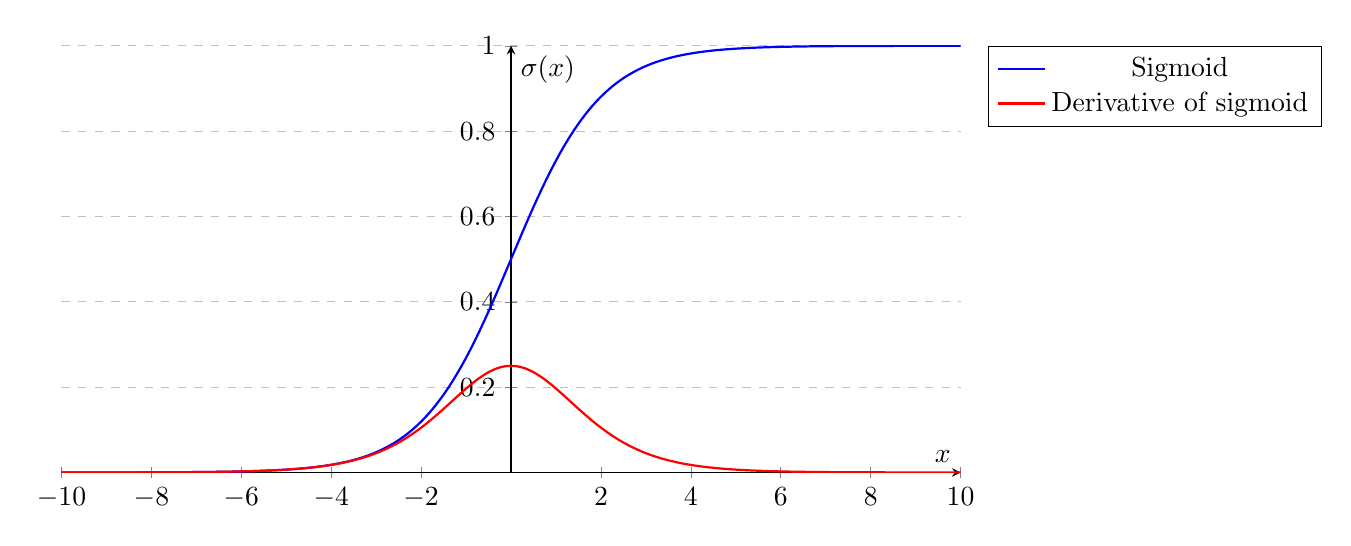
\begin{tikzpicture}
    \begin{axis}[
        axis lines=middle,
        xlabel={$x$},
        ylabel={$\sigma(x)$},
        xmin=-10, xmax=10,
        ymin=0, ymax=1,
        legend pos=outer north east,
        ymajorgrids=true,
        grid style=dashed,
        width=13cm, % Adjusted to your new width
        height=7cm, % Adjusted to your new height
    ]

    \addplot[
        color=blue,
        domain=-10:10,
        samples=100,
        smooth,
        thick,
    ]
    {1/(1+exp(-x))};
    \addlegendentry{Sigmoid}

    \addplot[
        color=red,
        domain=-10:10,
        samples=100,
        smooth,
        thick,
    ]
    {exp(x)/(1+exp(x))^2};
    \addlegendentry{Derivative of sigmoid}

    \end{axis}
  \end{tikzpicture}
  \caption{The sigmoid function and its derivative}
  \label{fig:Sigmoid}
\end{figure}

The sigmoid function is characterized by its distinctive S-shaped curve, serving as a pivotal nonlinear activation function in neural networks.\\
One of its notable features is the relationship between the input magnitude and the rate of change in the output. 
As the absolute value of the input escalates, the incremental change in the output significantly diminishes, leading to a derivative that approaches zero. 

Mathematically, the derivative of the sigmoid function, denoted as $\sigma'(x)$, can be expressed as:
\begin{equation}
\sigma'(x) = \sigma(x) \cdot (1 - \sigma(x)),
\end{equation}
where $\sigma(x)$ is the sigmoid function itself. 

In networks with a shallow architecture and fewer layers employing these activations, the vanishing gradient is less of an issue. 
However, the problem escalates with increased network depth, making the gradient too small for effective training.


\subsection{Long Short-Term Memory (LSTM) Networks}

LSTMs, as discussed by A. Graves et al.~\cite{graves2012long}, were designed to specifically address the challenges encountered with traditional RNNs, notably the vanishing gradient problem. 
Unlike standard RNNs, LSTMs incorporate a sophisticated gating mechanism to control the flow of information and gradients within the network.\\
This design significantly mitigates the vanishing gradient issue, enabling the network to learn from and remember information over extended sequences more effectively.
\newpage
The figure below illustrates the internal structure of an LSTM cell, showcasing its unique components:

\begin{figure}[ht]
  \centering
  \includegraphics[scale=0.2]{Figures/Chapter4/lstm_schematic_improved-transformed.png}
  \caption[LSTM Cell Structure]{LSTM Cell Structure}
  \label{fig:LSTM Cell Structure}
    
\end{figure}

LSTM cells include three critical gates: the input gate, the forget gate, and the output gate. 
These gates collectively manage the cell's memory, determining what information to retain, discard, and output. \\
This gating mechanism is pivotal for the LSTM's ability to modulate the gradient flow during backpropagation, directly addressing the vanishing gradient problem by maintaining gradient magnitude across long sequences.
The LSTM cell's core components are as follows:

\begin{itemize}

\item  \textbf{Forget Gate :}The forget gate plays a vital role in the LSTM architecture by deciding which information from the cell state should be kept or forgotten. It employs a sigmoid function to generate values between 0 and 1, with these values indicating the extent to which information is preserved or discarded.\\ 
This selective memory process enables LSTMs to focus on relevant information while minimizing unnecessary data retention, aiding in the preservation of gradient significance.

\item  \textbf{Input Gate and Output Gate :}The input gate is responsible for updating the cell state with new information. It operates in two steps: a sigmoid layer determines which values will be updated, and a tanh layer generates new candidate values.
 Conversely, the output gate decides what the next hidden state should be, which includes the filtered cell state information to be used in output.\\ 
 These gates ensure the network's ability to capture essential details for the task at hand, enhancing its long-term dependency modeling capabilities.

The operation of both the input and output gates ensures that if the outcome of these gates is close to 1, gradients can pass through without significant attenuation.Conversely, outcomes near 0 block the gradient flow. \\
This dynamic allows LSTMs to mitigate the vanishing gradient problem effectively.

\item  \textbf{Memory Cell State :}The memory cell state is the core component that allows LSTMs to retain information across time steps. It integrates inputs from the current time step and previous cell state, facilitating the network's ability to maintain a continuous flow of relevant information through the sequence. \\
The additive nature of the cell state updates helps to sustain gradient flow across long sequences, ensuring that LSTMs can capture and leverage long-range dependencies in the data.

\end{itemize}

\begin{itemize}
  \item \textbf{Forget Gate:} The forget gate plays a vital role in the LSTM architecture by deciding which information from the cell state should be kept or forgotten. It employs a sigmoid function to generate values between 0 and 1, with these values indicating the extent to which information is preserved or discarded.
  \[
  f_t = \sigma(W_f \cdot [h_{t-1}, x_t] + b_f)
  \]
  This selective memory process enables LSTMs to focus on relevant information while minimizing unnecessary data retention, aiding in the preservation of gradient significance.

  \item \textbf{Input Gate:} The input gate is responsible for updating the cell state with new information. It operates in two steps: a sigmoid layer determines which values will be updated, and a tanh layer generates new candidate values.
  \[
  i_t = \sigma(W_i \cdot [h_{t-1}, x_t] + b_i)
  \]
  \[
  \tilde{C}_t = \tanh(W_C \cdot [h_{t-1}, x_t] + b_C)
  \]
  Conversely, the output gate decides what the next hidden state should be, which includes the filtered cell state information to be used in output.

  \item \textbf{Cell State Update:} The memory cell state is the core component that allows LSTMs to retain information across time steps. It integrates inputs from the current time step and previous cell state, facilitating the network's ability to maintain a continuous flow of relevant information through the sequence.
  \[
  C_t = f_t \ast C_{t-1} + i_t \ast \tilde{C}_t
  \]
  The additive nature of the cell state updates helps to sustain gradient flow across long sequences, ensuring that LSTMs can capture and leverage long-range dependencies in the data.

  \item \textbf{Output Gate:} Determines the next hidden state, which includes the filtered cell state information to be used in outputs. The operation of the output gate ensures that gradients can pass through effectively, making it a key component in mitigating the vanishing gradient problem.
  \[
  o_t = \sigma(W_o \cdot [h_{t-1}, x_t] + b_o)
  \]
  \[
  h_t = o_t \ast \tanh(C_t)
  \]
\end{itemize}

\subsection{LSTM Intent Recognition Architecture}


 The application of theoretical approaches to intent recognition necessitates an investigation into various methodologies, with a particular focus on Long Short-Term Memory (LSTM) networks. 
 As detailed by Shao-Wen Wu et al.~\cite{wu2019predicting}, LSTM networks excel at understanding the complex patterns in data indicative of human intent. \\
 This research employs LSTM networks to estimate the parameters of a Beta distribution, demonstrating the networks' proficiency in accurately predicting human intentions, even in scenarios of incorrect teleoperation or obstacle avoidance, thus underscoring the model's dependability.

 Despite the effectiveness and reliability of this approach, it is not devoid of limitations. 
 A significant constraint is the assumption that objects remain stationary within their initial training environment. \\
 Any movement of these objects outside the direct view of the camera compromises the reliability of the alpha and beta parameters of the Beta distribution, leading to diminished accuracy in predictions.
 
In response to these impediments,in this thesis, the network will be assume the role of a binary classifier. 
This model, through the analysis of the end effector's distance and direction relative to an object, determines the likelihood of the object being the intended target for grasping. \\
Such an approach not only permits the LSTM to discern the complex dynamics between the input and output parameters, thereby enhancing its generalization capabilities, but also enables the adaptation of the model to accommodate the displacement of objects within the spatial domain without necessitating retraining.

Furthermore, the introduction of modularity into the model represents a significant advancement; by dedicating a distinct LSTM to each object, as show in figure ... the framework achieves scalability, allowing for its replication across multiple objects within a scene. \\
\begin{figure}[H]
  \centering
  
  \includegraphics[scale=0.5]{Figures/Chapter4/lstm_modularity.png}

  \caption{LSTM Model Modularity}
  \label{fig:LSTM Model Modularity}
\end{figure}




This characteristic ensures the model's viability in real-world scenarios, which are typified by the simultaneous presence of multiple objects, though it also necessitates an acknowledgment of the potential limitations posed by environmental clutter and computational resource constraints.

Central to this enhanced methodological approach is the objective of minimizing the model's inherent bias, thereby granting the LSTM the autonomy to independently identify and learn the subtle interrelations between distance and direction and their impact on object identification. 
This capacity for autonomous learning is imperative for the development of an intent recognition system that is not only efficient and adaptable but also robust enough to operate effectively within the complexities of real-world environments.\\
\newpage

Below a schematic of the LSTM model architecture is shown:

\begin{figure}[H]
  \centering
  \begin{tikzpicture}[
    node distance=1 cm and 0.5 cm,
    block_inout/.style={
      rectangle,
      draw,
      fill=yellow25,
      text width=1.5cm,
      align=center,
      minimum height=1cm,
      minimum width=3cm
    },
    block_lstm/.style={
      rectangle,
      draw,
      fill=orange25,
      text width=0.5 cm,
      align=center,
      minimum height=6cm,
      minimum width=0.55cm,
    },
    block_dp/.style={
      rectangle,
      draw,
      fill=green25,
      text width=0.5cm,
      align=center,
      minimum height=6 cm,
      minimum width=0.55cm,
    },
    block_dens/.style={
      rectangle,
      draw,
      fill=blue25,
      text width=0.5cm,
      align=center,
      minimum height=6cm,
      minimum width=0.55cm,
    },
    block_act/.style={
      rectangle,
      draw,
      fill=purple25,
      text width=0.5cm,
      align=center,
      minimum height=6cm,
      minimum width=0.55cm,
    },
    line/.style={draw, ->} % Define line style if needed
  ]

  % Nodes
  \node [block_inout] (input1) {distance};
  \node [block_inout, below=of input1] (input2) {direction};

  \node (distanceinput) at (2,0) [inner sep=0,minimum size=0] {};
  \node (directioninput) at (2,-2) [inner sep=0,minimum size=0] {};
  \node (center) at (1.5,-1) [inner sep=0,minimum size=0] {};


  \node [block_lstm, right=of center ] (lstm) {\rotatebox{90}{LSTM (100)}};
  \node [block_lstm, right=of lstm] (lstm1) {\rotatebox{90}{LSTM (50)}};

  \node [block_dp, right=of lstm1] (dropout1) {\rotatebox{90}{Dropout (0.25)}};
  \node [block_dens, right=of dropout1] (dense1) {\rotatebox{90}{Dense (20)}};
  \node [block_act, right=of dense1] (activation1) {\rotatebox{90}{Act (tanh)}};
  
  \node [block_dp, right=of activation1] (dropout2) {\rotatebox{90}{Dropout (0.25)}};
  \node [block_dens, right=of dropout2] (dense2) {\rotatebox{90}{Dense (1)}};
  \node [block_act, right=of dense2] (activation2) {\rotatebox{90}{Act (sigmoid)}};

  \node [block_inout, right=of activation2] (output1) {pick\\ probability};
 

  % Arrows
  \draw[line] (input1.east) -- (distanceinput.west);
  \draw[line] (input2.east) -- (directioninput.west);
  \draw[line] (lstm) -- (lstm1);
  \draw[line] (lstm1) -- (dropout1);
  \draw[line] (dropout1) -- (dense1);
  \draw[line] (dense1) -- (activation1);
  
  \draw[line] (activation1) -- (dropout2);
  \draw[line] (dropout2) -- (dense2);
  \draw[line] (dense2) -- (activation2);
  \draw[line] (activation2) -- (output1);


\end{tikzpicture}
  \caption{LSTM Model Architecture}
  \label{fig:LSTM Model Architecture}
\end{figure}

To arrive a this final model, it was vital to carfelly plan evry step of the process, from the pre-processing of the data to modelling of each layer of the network.\\
since a minor change in the architecture of the network can lead to a significant change in the performance of the model, it was important to carefully plan each step of the process.\\

\paragraph{Pre-Processing of the Data}

The initial step in developing the model involved setting the number of neurons for the first LSTM layer. 
The LSTM, being a recurrent neural network, processes inputs sequentially through its repetitive cell structure. 
This means each cell within the layer handles a distinct input from the time sequence; specifically, as showcased in figure \label{RNN_single_layer}, the first cell processes the first input, the second cell the second input, and so on.

Selecting the appropriate number of cells in this layer is crucial. 
This choice is one of the first and most significant hyperparameters to be determined, directly impacting the model's capacity and computational demands.
Once this hyperparameter is established, it sets a foundational aspect of the model's architecture that is not easily modified later.

Analysis of data from 26 teleoperation experiments revealed an average of 2820 timesteps per experiment, with each experiment lasting around 26 seconds on average. 
Given this data, and to efficiently balance model complexity with the available computational resources, the neuron count for the first layer was set to 100. 

\paragraph{Stacked LSTM}

Recent studies on the application of Long Short-Term Memory (LSTM) networks to time series data, highlighted by \cite{cui2019deep} and \cite{9096332}, have revealed the efficacy of employing stacked LSTM layers in enhancing model performance. 
This design approach facilitates hidden layers in capturing progressively higher-level representations of the sequence data. 
Deep LSTM models, characterized by multiple LSTM hidden layers, create a structured flow where the output of one layer directly feeds into the subsequent layer, thereby significantly boosting the neural network's (NN) capability to learn. 

The hyperparameter configuration for modeling complex relationships was determined to be a two-layer LSTM structure. 
This choice was guided by the recognition that, although additional layers may enhance the model's ability to identify complex relationships among feature variables, a point is reached where further layers contribute to diminishing returns and increased risk of overfitting. Considering the dataset characterized by a relatively small number of input timesteps, incorporating a third layer would likely lead to overfitting, undermining the model's generalizability and efficiency.

\paragraph{Other layers}

To further mitigate the risk of overfitting in models with multiple layers, such as stacked LSTM networks, dropout layers have been introduced. 
This method involves randomly removing a specified proportion of neurons, as determined by the dropout ratio, from the network during each training iteration, effectively preventing their contributions to downstream neuron activation and halting weight updates during backpropagation for that iteration. For this experiment, the dropout ratio was set to 0.25, meaning 25\% of neurons in a layer are ignored at each training step, reducing the model's dependence on specific neurons and encouraging the learning of more robust features through forced feature redundancy. 
This approach not only helps in spreading out weights to diminish the likelihood of overfitting but also ensures the model does not rely too heavily on a small set of neurons, thereby improving its ability to generalize to unseen data. 
It is crucial to note that dropout is applied exclusively during training, with all neurons active during testing or evaluation phases, although their outputs are adjusted by the dropout rate to maintain consistency with the training environment

\begin{figure}[H]
  \centering
  
  \includegraphics[scale=0.4]{Figures/Chapter4/Droput.png}

  \caption{Effect of Dropout layer}
  \label{fig:Dropout}

\end{figure}

Another crucial part of the model, is th Fully-Connected layer, often referred to as a Dense layer in neural networks, which ensures complete interconnectivity between the neurons of consecutive layers. 
In such a layer, each neuron from the previous layer is linked to every neuron in the next, facilitating the layer's ability to derive a comprehensive linear combination of the input features. 
This configuration is instrumental in the network's capability to discern complex patterns within the depth of neural network models.\\
As seen in the stacked LSTM, which saw a reduction of cell from 100 to 50, the first Dense layer was configured to contain 20 neurons. 
This configuration aims to refine the feature space, enabling the network to concentrate on the most significant patterns identified by the LSTM layers, culminating in a final output layer comprising a single neuron. 
Both the LSTM and Dense layers employ the \textit{tanh} activation function.\\
The \textit{tanh} function is frequently chosen for LSTM layers due to its effectiveness in capturing complex patterns by introducing non-linearity into the network. 
Non-linearity is essential, as a purely linear model would be incapable of recognizing the intricate patterns present within the data.

Given the model's objective to classify the intention to pick or not pick an object based on the input, the task falls within the scope of a binary classification problem. 
Therefore, the architecture necessitates the inclusion of a Dense layer as the final component, distinguished by a single neuron utilizing a 'sigmoid' activation function. 
The 'sigmoid' function, characterized by its output range extending from 0 to 1, permits this concluding layer to map the features refined by antecedent layers into a predictive probability. 
This calculated probability serves to articulate the model's confidence in categorizing the input under one of two potential outcomes: the action to pick or the decision against picking the object.

\paragraph{Implementation of the model}
To deploy the LSTM model, it was done in python, more specifically using the keras library
Keras \cite{chollet2015keras} is a Python-based, open-source library designed to facilitate the development and training of deep learning models efficiently.
Acting as an interface for TensorFlow, it simplifies complex processes with predefined layers and algorithms for rapid experimentation. 
Emphasizing user-friendliness and modularity, Keras supports various backend engines, operates on both CPUs and GPUs, and enables quick prototyping with minimal code. 
This makes it accessible to users at all levels in the fields of machine learning and artificial intelligence.


'CODE?'





\subsection{Training the model}








